\documentclass[a4paper,10pt]{article} 

\usepackage[utf8]{inputenc} 
%\usepackage[T1]{fontenc}

\usepackage{textcomp}           % Extra Symbole (Grad Celsius etc.)
\usepackage{amssymb,amsmath}    % Schöne Formeln (AMS = American Mathematical Society)
\usepackage{graphicx}           % Bilder und Seitenränder
\usepackage{subcaption}			% captions for subfigures
\usepackage{booktabs}           % Schönere Tabellen
\usepackage{colortbl}           % Farbige Tabellen

%\usepackage{tcolorbox}			% schöne bunte Boxen
\usepackage{mathtools}			% \mathclap für ordentliche \underbrace-			environments
\usepackage{geometry}			% Pagelayout mit \newgeometry, \restoregeometry
\usepackage{float}
\usepackage{wrapfig}
\usepackage{enumitem}
\usepackage{float}
\usepackage{braket}
\usepackage{caption}

\graphicspath{{./img/}}


\bibliographystyle{unsrtnat}

\renewcommand{\k}{\mathbf{k}}
\begin{document}
\begin{titlepage}
 \begin{center}
	\Large{Advanced laboratory class 3}
	\end{center}
	\begin{center}
	 \LARGE{\textbf{FP3 - SQUID}}
	\end{center}
	
	\begin{center}
	
	\large Marco \textsc{Canteri} \\
	marco.canteri@student.uibk.ac.at
	\end{center}
	
	\begin{center}
	\vspace{1cm}
	Innsbruck, \today
	\vspace{2cm}
	\end{center}
	
	\begin{center}
	
\includegraphics[scale=0.4]{img/uibk} 
	\end{center}

\end{titlepage}
\begin{abstract}

\end{abstract}
\section{Introduction}
\section{Theory}
\subsection{Superconductivity}
Superconductivity is the property of a medium to conduct current without any resistance. It was first discovered in 1911, when Heike Onnes cooled down mercury below 4.2 K \cite{firstsuperconductor}, finding out that the resistance dropped to zero. Since this discovery, superconductivity has been discovered in many elements and media which resistance drops to zero below a particular critical temperature $T_c$. There are different ways to classify superconductors, the easiest one is to divide superconductors in low-$T_c$ and high-$T_c$ superconductors. Low temperature superconductors are material with a critical temperature below $30$ K, while high temperature superconductors have $T_c$ greater than 30 K.\\
Superconductors can lose their property of superconductivity not only with a change in temperature, but also with a change of magnetic field or current, this leads to a different classification of superconductors: type I and type II superconductors. The former has a critical external magnetic field $H_c$ and behaves as superconductor below this field. Type II superconductors have two different critical fields, and they behave differently in various regimes.\\
In this experiment we used a Yttrium barium copper oxide (YBCO) superconductor which is a high-$T_c$ superconductors, historically is also the first high-$T_c$ superconductors found with a critical temperature above 77 K, the boiling point of liquid nitrogen. Indeed the critical temperature of YBCO is around 90-94 K, depending of the compound and purity.\\
The theoretical description of superconductivity can be done in different ways, the first classical approach is the simplest description using London equations, a quantum mechanical formulation is the Ginzburg-Landau (GL) theory which describes the macroscopic properties of superconductors. However this theory is still phenomenological, the first microscopic model is the BCS theory which was able to describe superconductivity from a microscopic point of view and has the GL theory as a limit. The key idea of BCS theory is that at low temperatures electrons pair up and form Copper pairs, creating a bosonic condensate. This condensate must be described as a single entity with a wavefunction $\psi(\mathbf{r},\theta) = |\psi(\mathbf{r})| e^{i\theta}$, which is not normalized, but $|\psi(\mathbf{r},\theta)|^2 = n_e$, where $n_e$ is the number of electrons in the superconductive state. These theory predicts the behaviour of low temperature superconductors, but fails to describe high temperature superconductors, whose description is still an open problem.


\subsection{Josephson effect and SQUID}

\section{Experiment setup}
\subsection{Shapiro steps and $e/h$}
In order to observe Shapiro steps, we inserted an antenna inside the dewar such that we coupled electromagnetic radiation with the squid. The antenna was connected to a function generator with we used to generate a sine wave whit variable amplitude and frequency. With this setup we acquired again the characteristic V-I curve of the SQUID for five different frequencies ranging from 10 to 20 GHz. After setting the desired frequency we changed the power of the wave such that the Shapiro steps were maximized.
\subsection{Critical temperature measurement}
To measure the critical current of the SQUID we measured the resistance at various temperatures. To measure the temperature we build the circuit in figure \ref{circuit}. The REF02 provides us with a stable voltage of approximately 5V, we chose resistor $R_1 \simeq 40$ k$\Omega$ and $R_2 \simeq 10$ k$\Omega$ such that the voltage at the non inverting input of the opamp is around 1V. For the last resistor  we chose $R_3 \simeq 80$ k$\Omega$, thus the fixed current was approximately 12 mA. The diode was attached to the squid, hence we were able to measure a difference in temperature by measuring the voltage across the diode. To calibrate this circuit we took two points, one at the boiling point of the nitrogen (77 K) and the other one at room temperature, such that we had a direct conversion from voltage to temperature.\\
To measure the resistance of the SQUID we acquired the characteristic V-I curve whose slope gives the resistance. We proceeded to slowly lower the squid into the liquid nitrogen, such that the gradient of temperature between the liquid nitrogen and the environment would give us different points with different temperatures. During the lowering we stopped several times to take the measurements, every time we waited several minutes until voltage on the multimeter was stable and then we acquired the resistance and wrote down the voltage on the multimeter.
We took several point with different spacing, more densly near the critical temperature at 90 K and more rarely at higher temperature until the squid was completely inside the liquid nitrogen and therefore at 77 K.
\begin{figure}[H]
\centering
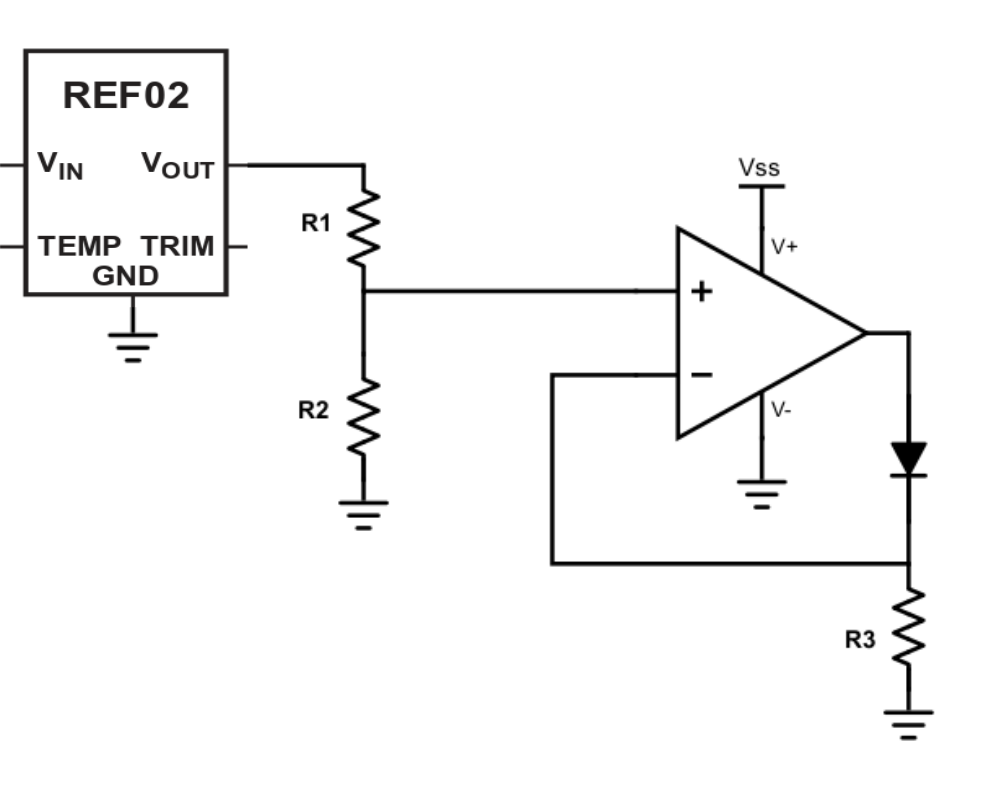
\includegraphics[width = .5\textwidth]{circuit}
\caption{Circuit for current source used to measure the temperature}\label{circuit}
\end{figure}
\section{Analysis}
\subsection{Shapiro steps and $e/h$}
\subsection{Critical temperature measurement}
 \begin{thebibliography}{99}
\bibitem{firstsuperconductor} \textsc{H. K. Onnes} \textit{The resistance of pure mercury at helium temperatures}, Commun. Phys. Lab. Univ. Leiden, Vol. 12 (1911), 120 

\bibitem{skriptum} Fortgeschrittenenpraktikum 2, \textit{Entanglement and Bell’s inequality}. \textsc{Gregor Weihs, Kaisa Laiho, Harishankar Jayakumar}. WS 2015/16
\end{thebibliography}
\end{document}
